\chapter{The Stability of FLUTE the Electron Gun and Proposed Stabilizing Solution}
This chapter deals with the electron gun of \gls{flute} and its power supply. Then based on fundamental equations of electron gun's microwave cavity, the dependence of the electron energy from the \gls{rf} supply is derived, which motivates why the \gls{rf} supply should be stable. Then a solution to stabilize the \gls{rf} is proposed.

The electron gun is powered by a \SI{50}{\MW} klystron, a high-power vaccum tube \gls{rf} amplifier. The input signal for the klystron is a \SI{2.99855}{\GHz} harmonic oscillator pre-amplified to \SI{200}{\watt}. The supply input is generated by a pulse forming network and a transformer. The pulse forming network mainly consists of capacitors to store electrical energy and is charged with a constant current source. The connection of these devices is shown in \autoref{fig:fluteEgun-rfschematic}.

A \SI{5}{\hertz} master clock (``trigger'') is used to switch on the output of the pulse forming network to the klystron and the oscillator every \SI{0.2}{\second} for \SI{4.5}{\micro\second}. During this time, the laser could also be triggered causing a stimulated emission of an electron bunch from the cathode. But even without the laser being active, powering the electron gun with the klystron generates an electron beam through thermionic emission of electrons. This undesired effect is called \textit{dark current}.

The current source to charge the pulse forming network is powered by mains voltage. This makes it susceptible to noise on the mains and also caused slowly time varying drifts of the klstron power due the pulse forming network being triggered at different relations to the mains \SI{50}{\hertz}. This issue has been remedied in \cite{Nasse2019} by adding synchronization to the mains phase.

\begin{figure}[tb]
	\centering
	\includegraphics[]{chap/StabilityOfTheElectronGun/img/fluteSchem.tikz}
	\caption{Schematic of the \gls{flute} \gls{rf} system}
	\label{fig:fluteEgun-rfschematic}
\end{figure}

\section{The Electron Gun}
The electron gun of \gls{flute} was originally designed and operated in CTF II at \gls{cern}. \cite{Schuh2014}
It is of the ``BNL type'' (see \cite{Batchelor1988}, based on the original design by \cite{fraser1987}) and was  developed at \gls{cern}. \cite{Bossart:288412}

The gun is made up of a 2.5 cell microwave cavity with a removable copper cathode embedded in the cone shaped back at the end of the half cell (see \autoref{fig:fluteEgun-gunDraw}). Cooling is achieve with a two-stage water cooling system: A temperature control unit uses a short water circuit to cool the gun while itself uses a heat exchanger to a bigger outside climate unit.

Applying \gls{rf} power to the cavity through the hole-coupled wave guide causes a standing wave inside the cavity. Because of the cavity's dimensions, only the fundamental mode $\text{TM}_{010}$ is excited, for which the relation between resonance frequency $f_{010}$ and radius $a$ of the cavity is given by
\begin{equation}
\frac{f_{010}}{2\pi}=\frac{2.405 \cdot c}{a}.
\end{equation}
For the $\text{TM}_{010}$ mode there is only an electrical field in the $z$ direction, i.e. along the beam axis. This $E_z(z)$ field is used to accelerate the electrons. For the \gls{flute} gun, $E_z(z)$ has been measured in \cite{Bossart:clic}, see \autoref{fig:fluteEgun-Ezplot}. These measurements are also verified in \cite{Schuh2014}.

To tune the resonance frequency $f_{010}$, which depends on the cavity's radius $a$, to the target design frequency of \SI{2.99855}{\GHz}, two method are used. For once the cavity is equipped with piston tuners that allow changing the geometries of each cell slightly. Additionally because of the expansion and contraction of the copper body due to temperature changes, the set-point of the water cooling system can also be changed to alter the cavity geometry.

\begin{figure}[tbh]
	\centering
	\includegraphics[width=\textwidth,height=0.5\textwidth]{chap/StabilityOfTheElectronGun/img/Ez.tikz}
	\caption{Plot of the electrical field in $z$ direction over the length of the gun cavity (redrawn from \cite{Bossart:clic} using geometrical measurements from \cite{Hoeninger2014})}
	\label{fig:fluteEgun-Ezplot}
\end{figure}

\begin{figure}[tbh]
	\centering
	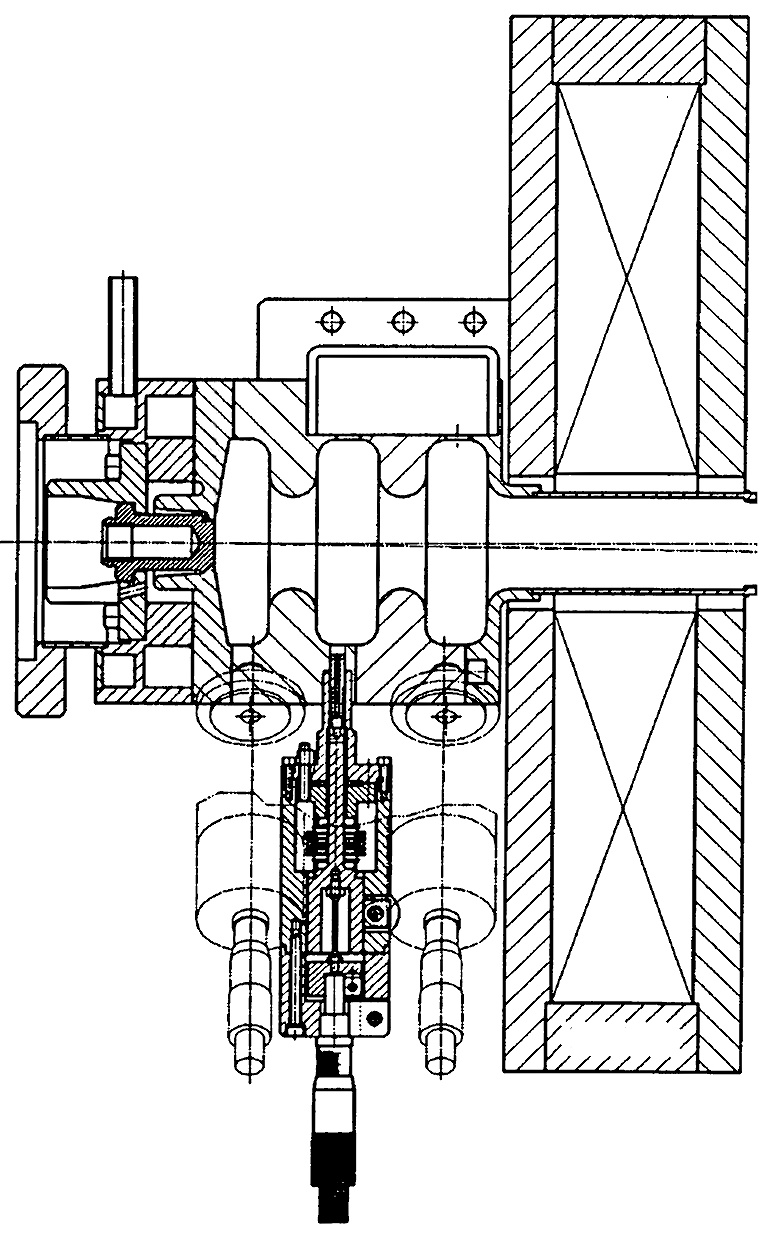
\includegraphics[]{chap/StabilityOfTheElectronGun/img/gun.tikz}
	\caption{Cross section drawing of the electron gun together with the solenoid (which is used for focusing the electron beam) showing the photo-cathode (red) and the electron and laser beam trajectories
	\\(modified version from \cite{Bossart:clic} and \cite{Bossart:288412})}
	\label{fig:fluteEgun-gunDraw}
\end{figure}


\section{Relation between RF power and Electron Energy}
A standing wave inside a \gls{rf} cavity for a $TM_{010}$ mode can be written as
\begin{equation}
E_z(z,t) = E(z)\,\cos(\omega t + \phi).
\end{equation}
The time $t$ has to be expressed in terms of the electron velocity $v(z)$ as
\begin{equation}
t=t(z)=\int_{0}^{z} \frac{\d{z}}{v(z)},
\end{equation}
which is the arrival time of the electron at location $z$.

If moving through an accelerating gap of length $L$ inside a cavity, an electron with charge $q$ gains the energy
\begin{equation}
\Delta W = q \int_{-L/2}^{L/2} E(z)\,\cos(\omega t(z) + \phi) \d{z}
\end{equation}

This can be rewritten as
\begin{equation}\label{eq:W}
\Delta W = q V_0 T \cos(\phi)
\end{equation}
using the axial \gls{rf} voltage
\begin{equation}
V_o := \int_{-L/2}^{L/2} E(z) \d{z}
\end{equation}
and the travel time factor $T$. \cite[p.~32]{Wangler2008}

With the \textit{shunt impedance} $R_s$, the axial \gls{rf} voltage can be brought into relation with the \gls{rf} power, that need to be induced into the cavity to compensate losses in the non-perfect conducting walls and power lost to the electron beam. \cite{burtRF}

The shunt impedance is defined as
\begin{equation}\label{eq:rs}
R_s = \frac{V^2_0}{P_{\text{RF}}} 
\end{equation}

\autoref{eq:W} and \autoref{eq:rs} show that the \gls{rf} supply has a great impact on the electron energy, so it needs to be stable.

Additionally, there is the so called \textit{R over Q}, defined as
\begin{equation}
\frac{R}{Q} = \frac{(V_0T)^2}{\omega U}\qquad \text{with: }R=R_s T^2\;\text{(effective shunt impedance)}
\end{equation}
using the total stored electromagnetic energy $U$ and the quality factor $Q=\nicefrac{\omega U}{P_{\text{RF}}}$.

This shows the gained energy also depends on the properties of the cavity.

\section{Current RF Stability and Proposed Solution}
To get an overview of the current stability of the \gls{rf} power, the deviation of the cavity power process value (\gls{epics}: F:RF:LLRF:01:GunCav1:Power:Out Value) from its mean is plotted over one hour, see \autoref{fig:fluteEgun-deviation}.


With the metrics defined in \autoref{sec:metrics}, the $\op{\%STD}$ is \SI{0.15}{\percent} and the $\op{MSE}$ is \num{38.54}.

From the time plot in \autoref{fig:fluteEgun-deviation} and the periodogram in \autoref{fig:fluteEgun-periodo} it becomes clear that there is random white noise, but also a periodic part and a slow drift in the signal. While it is not possible to counteract the random fluctuations be any practical means, it is however possible to compensate for the slower disturbances.

Hence in the next chapters, the control system is developed to counteract these noise components. 

The control system should be made up with a controllable \gls{rf} attenuator added to the existing \gls{rf} system. This way there is no modification to the proprietary \gls{llrf}\footnote{The \gls{llrf} is visualized as only the oscillator in \autoref{fig:fluteEgun-rfschematic} and \autoref{fig:fluteEgun-rfschematicControl} but contains also its own feedback system and a vector modulator} necessary. With the addition of the control unit (see \autoref{fig:fluteEgun-rfschematicControl}), which is designed in later chapters and contains the controller $G(s)$ and the filter $H(s)$, the a closed-loop for feedback control is formed.

\begin{figure}[tb]
	\centering
	\includegraphics[]{chap/StabilityOfTheElectronGun/img/fluteSchemControlUnit.tikz}
	\caption{Schematic of the \gls{flute} \gls{rf} system with the proposed control unit and the controllable \gls{rf} attenuator added}
	\label{fig:fluteEgun-rfschematicControl}
\end{figure}

\begin{figure}[tb]
	\centering
	\includegraphics[width=\textwidth,height=0.5\textwidth]{chap/StabilityOfTheElectronGun/img/assesment.tikz}
	\caption{Deviation of the cavity \gls{rf} power over the course of one hour}
	\label{fig:fluteEgun-deviation}
\end{figure}

\begin{figure}[tb]
	\centering
	\includegraphics[width=\textwidth,height=0.5\textwidth]{chap/StabilityOfTheElectronGun/img/periodo.tikz}
	\caption{Periodogram of \autoref{fig:fluteEgun-deviation}; calculated using the Welch method}
	\label{fig:fluteEgun-periodo}
\end{figure}




